\chapter{IEC 61850 -standardi}
\label{ch:iec61850-theory}
% Aihepiirijärjestys tutusta uuteen.
% Tuttuja asioita: sähköasema, julkaisija-tilaaja-paradigma, viestejä voidaan tilata.
% Luvussa käsiteltävät asiat.
IEC 61850 -standardi määrittää säännöt, kuinka sähköaseman laitteet kommunikoivat keskenään verkon yli \cite[s.~1]{Kaneda2008}. Standardi koskee myös aseman kanssa kommunikoivia ohjelmistoja \cite[s.~10]{IEC61850-7-1}. Standardi on laaja monesta dokumentista koostuva kokonaisuus. Tämän takia tässä luvussa standardista käsitellään vain diplomityön kannalta tärkeitä asioita. Käsittely aloitetaan yleiskuvalla ja edetään tärkeään asiaan. Saatuja tietoja tullaan käyttämään myöhemmin pohjana järjestelmän arkkitehtuurin ja ohjelmiston suunnittelussa.


\section{Yleiskuva}
% Sähköaseman IED-laitteet toteuttavat aseman toiminnallisuutta.
Sähköaseman tehtäviin kuuluu mm. jännitteen muuntaminen, verkon jakaminen ja sen toiminnan tarkkailu. Virhetilanteissa aseman laitteisto toimii estääkseen suuremman vahingon. Näitä laitteita sähköasemalla ohjaa ja tarkkailee sen automaatiolaitteet, joita kutsutaan \emph{älykkäiksi elektroniikkalaitteiksi} (\emph{Intelligent Electronic Device}, \emph{IED}). IED:t ovat kytketty sähköverkon laitteisiin joita ne ohjaavat \cite[s.~63--64]{IEC61850-7-1}. Näitä laitteita on mm. muuntajat ja katkaisijat. IED:t myös kytketään verkkoon, jotta ne voivat kommunikoida keskenään ja asemalta ulospäin \cite[s.~31]{IEC61850-7-1}. Asemalta ulospäin kommunikointi mahdollistaa sen etäohjauksen ja tarkkailun ohjelmiston avulla \cite[s.~1]{Brunner2008}.

% Standardi IED-laitteiden kommunikoinnin määrittämiseen.
% Standardia voi toimia monella eri tekniikalla, mutta käytetään MMS-protokollan avulla.
IEC 61850 -standardi määrittää kuinka IED-laitteet ja etäohjelmistot kommunikoivat keskenään. Standardin tarkoitus on asettaa yhteiset säännöt, jotta eri valmistajien laitteet ja ohjelmistot olisivat yhteensopivia keskenään. Standardi on määritetty tekniikasta riippumattomaan muotoon, joka erikseen mallinnetaan halutulle tekniikalle \cite{IEC61850-1}. Mallinnuksia on olemassa eri tekniikoille, mutta tässä työssä kommunikointi tapahtuu pelkästään \emph{MMS}-protokollan (\emph{Manufacturing Message Specification}) päällä. MMS-protokolla on TCP/IP-protokollaperheen päällä toimiva kommunikointiprotokolla \cite{MMS-protocol-stack-and-API}.

% Viestien tilauksen pääpiirteinen toiminta.
Standardi määrittää säännöt kuinka asiakasohjelmat voivat tilata viestejä IED-laitteelta verkon yli. Viestien tilaus noudattaa julkaisija-tilaaja-paradigmaa, jossa IED-laite on julkaisija ja asiakasohjelmat tilaajia. Julkaisija-tilaaja-paradigma käsiteltiin aikaisemmin kappaleessa \ref{ch:julkaisija-tilaaja-paradigma}. Viestien sisältö on IED-laitteessa olevaa tietoa, kuten mittausdataa tai siihen kytketyn laitteen tilatietoa. Viestit tilataan IED-laitteelta olevalta oliolta, joka konfiguroidaan ennen tilausta. Standardi asettaa rajoituksia tilaajien määriin, jotka täytyy ottaa huomioon ohjelmiston suunnittelussa. Jotta näitä rajoituksia ja tilauksen toimintaa voidaan ymmärtää, täytyy ensin tarkastella, kuinka standardi määrittää muuttujia IED-laitteeseen. \mbox{\cite[s.~91--97]{IEC61850-7-2}}


\section{Sähköaseman laiteiden mallinnus}
% Muuttujilla IED-laite mallintaa aseman laitetta.
Muuttujilla IED-laite mallintaa siihen kytkettyä sähköaseman laitetta kuten katkaisijaa tai muuntajaa. Muuttujat esittävät mm. linjasta mitattua jännitteen arvoa tai katkaisijan tilaa, joka voi olla auki tai kiinni. IED-laitteessa olevien muuttujien määrä vaihtelee sen mukaan mitä laitetta sen on tarkoitus ohjata. \cite[s.~28]{IEC61850-7-1}

% Muuttujat muodostuvat valmiiksi määritetyistä luokista.
Mitä muuttujia IED-laite sisältää määrittyy standardin mukaan. Standardi esittää luokkamäärityksiä kaikille sähköaseman laitteille mm. katkaisijoille ja muuntajille. Luokka määrittää mitä muuttujia sen instanssi tulee sisältämään ja jotka kuvaavat kyseistä laitetta. Luokasta muodostetaan instanssi IED-laitteelle sen mukaan, mitä laitetta se ohjaa. Esimerkiksi jos IED-laite ohjaa linjan katkaisijaa, määritetään IED-laitteeseen standardin määrittämä katkaisijaluokan instanssi. Tällöin IED-laite sisältää muuttujia katkaisimen tilasta ja sen ohjauksesta. \cite{IEC61850-7-3, IEC61850-7-4}

% Luokkat muodostavat hierarkian ja koostuvat toisistaan.
Standardin luokkamääritykset sisältävät aliluokkia ja jotka taas sisältävät muuttujia tai muita aliluokkia. Standardissa luokkamääritykset toimivat samalla periaatteella kuin oliohjelmoinnin luokat. Luokat sisältävät samaan asiaan liittyviä muuttujia ja toiminnallisuutta. Näistä luokista ja muuttujista standardissa muodostuu oliopohjainen hierarkkinen rakenne. Esimerkiksi muuntajaa mallintava luokka sisältää aliluokkia mittaustiedon esittämisestä. Samaa aliluokkaa käytetään jonkin muun mittaustietoa sisältävän laitteen mallintamiseen. Voidaan sanoa, että standardin mukainen laitteen luokka koostuu muista aliluokista. Kun laitteen mallintavasta luokasta tehdään instanssi IED-laitteelle, samalla myös tehdään instanssi kaikista sen aliluokista. IED-laite siis sisältää myös kaikki aliluokkien muuttujat. \mbox{\cite[s.~108]{IEC61850-7-1}}

\section{Muuttujien yksilöinti IED-laitteessa}
% Viittaus muuttujiin hierarkiassa.
IED-laite siis sisältää muuttujia hierarkiassa sen mukaan mitä laitetta se ohjaa. Näitä muuttujia voidaan lukea ja kirjoittaa standardin määrittämillä palvelukutsuilla. Jotta voidaan yksilöidä mitä muuttujia halutaan kutsulla lukea tai kirjoittaa, muuttujia täytyy pystyä yksilöimään hierarkiassa. Tätä varten standardi määrittää viittaustekniikan, jota käytetään kutsun yhteydessä yksilöimään mitä muuttujia se koskee. Tämä viittausformaatti on määritetty kuvassa \ref{fig:iec61850-data-reference}. Viittaus muodostuu hierarkiassa olevien luokkien instanssien ja muuttujien nimistä. Nimiä yhdistetään peräkkäin, jolloin viittausta voidaan seurata lukemalla minkä luokan instanssin mitä muuttujaa halutaan lukea tai kirjoittaa. Ensimmäisen ja toisen nimen väliin tulee kauttaviiva (/) ja loput yhdistetään pisteellä (.). \mbox{\cite[s.~625--626]{Mackiewicz2006}} \mbox{\cite[s.~93--95]{IEC61850-7-1}}

\begin{figure}[ht!]
	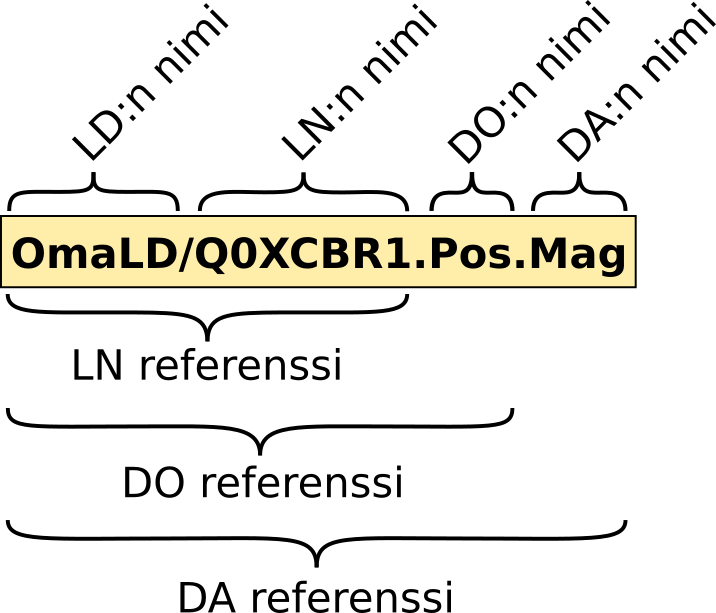
\includegraphics[width=0.5\textwidth]{pictures/iec61850-data-reference.png}
	\caption{IEC 61850 -standardin määrittämä viitteen rakenne (pohjautuu kuvaan \mbox{\cite[s.~93]{IEC61850-7-1}}).}
	\label{fig:iec61850-data-reference}
\end{figure}

% Viittauksen käsitteet lyhyesti.
Viite muodostuu käsitteistä:
\begin{itemize}
	\item \emph{looginen laite} (\emph{Logical Device}, \emph{LD}),
	\item \emph{looginen noodi} (\emph{Logical Node}, \emph{LN}),
	\item \emph{dataobjekti} (\emph{Data Object}, \emph{DO}) ja
	\item \emph{data-attribuutti} (\emph{Data Attribute}, \emph{DA}).
\end{itemize}
viitteessä vasemmalta oikealle järjestyksessä. Käsitteet ovat standardissa tapa esittää minkä tason luokka tai muuttuja hierarkiassa on kyseessä. Tämä tieto on diplomityön ulkopuolella ja lukija voi ne tarkistaa tarvittaessa standardista. Kuitenkin lyhyesti \emph{looginen laite} esittää jotakin aseman fyysistä kokonaisuutta, jota IED-laite ohjaa. \emph{Looginen noodi} on luokka laitteesta kuten muuntajasta tai katkaisijasta. \emph{Dataobjekti} on luokka joka sisältää muuttujia samaan asiaan liittyen, esimerkiksi mittaukseen. \emph{Data-attribuutti} on muuttuja, joka sisältää arvon mitatusta jännitteestä tai katkaisijan tilasta. \mbox{\cite[s.~2]{Camachi2017}} \mbox{\cite[s.~24]{IEC61850-1}}


\section{Viestien tilaus}
% Viestin tilauksen luokan toiminta.
Standardi määrittää luokkia eri asioiden mallintamiseen, joista tehdään instansseja IED-laitteelle tarpeen mukaan. Samaa periaatetta noudattaen standardi määrittää myös luokan, joka vastaa viestien tilauksesta. Standardissa luokkaa kutsutaan nimellä \emph{RCB} (\emph{Report Control Block}). Luokasta on tehty instanssi muuttujien hierarkiaan ja sillä on nimi. Luokan instanssi sisältää sisältää muuttujia tilauksen konfigurointiin, aloittamiseen ja lopettamiseen. Näitä muuttujia tilajaa voi kirjoittaa ja lukea palvelukutsuilla jotka viittaavaat RCB-luokan instanssiin. Esimerkki viitteestä RCB-instanssin arvojen kirjoittamiseen voi olla \emph{OmaLD/LLN0.BR.OmaRCB}. \mbox{\cite[s.~95--97]{IEC61850-7-2}}

% Viestiluokkien datajoukot.
RCB-instanssi vastaa tilaajan tilauksen konfiguroinnista ja viestien lähettämisestä. Sisältö viestiin tulee standardin määrittämistä \emph{datajoukoista} (\emph{data set}). IED-laitteelle on mahdollista määrittää standardin mukaisia datajoukkoja. Datajoukko on kokoelma IED-laitteella olevista muuttujista, jotka on kerätty yhteen niiden tärkeyden takia, esimerkiksi kaikki mittauspisteet voivat kuulua yhteen datajoukkoon. RCB-instanssi konfiguroidaan tarkkailemaan yhtä tällaista datajoukkoa, josta tilaaja on kiinnostunut. Datajoukossa tapahtuneen muutoksen myötä RCB-instanssi luo viestin, johon se sisällyttää muuttuneet arvot ja lähettää sen tilaajalle. Esimerkki tästä on jännitteen mitatun arvon muuttuminen uuteen, jonka tarkkaileva RCB-instanssi huomaa. Seurauksena instanssi luo uuden viestin, sisällyttää muuttuneet arvot viestiin ja lähettää sen tilaajalle. Sama toistuu minkä tahansa datajoukon muuttujan muuttuessa. \mbox{\cite[s.~93]{IEC61850-7-2}}

% Viestiluokan rajoitteet.
Standardi asettaa rajoitteita RCB-instanssiin. Yksi RCB-instanssi voi palvella vain yhtä tilaaja kerrallaan. Instanssi niin sanotusti varataan tilauksen aloitushetkellä, jolloin muiden tilaajien kirjoitus luokkaan estetään, niin kauan kunnes nykyinen tilaaja lopettaa tilauksen tai yhteys katkeaa. Monen tilaajan halutessa saman datajoukon tiedot muutoksista, täytyy IED-laitteeseen määrittää RCB-instansseja tarpeen mukaan ja konfiguroida ne tarkkailemaan samaa datajoukkoa \cite[s.~93]{IEC61850-7-2}. Kuvassa \ref{fig:rcb-to-one-dataset} on esitetty tilanne, jossa kolme tilaaja tilaavat saman datajoukon käyttäen kolmea eri RCB-instanssia. Kuvassa neljäs tilaaja ei voi kirjoittaa jo varattua isntanssia, joten sen ei ole mahdollista tilata datajoukosta tulevia viestejä.

\begin{figure}[ht!]
	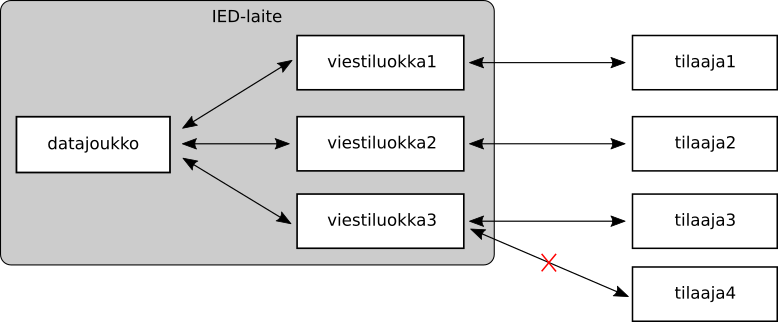
\includegraphics[width=1\textwidth]{pictures/rcbs-to-one-dataset.png}
	\caption{Kolme RCB-instanssia IED-laitteessa palvelee kolmea tilaajaa samasta datajoukosta.}
	\label{fig:rcb-to-one-dataset}
\end{figure}


\section{Viestien sisältö}
% Viestin sisältö koostuu yleisistä tiedoista ja taulukosta arvoja.
Tilaaja siis tilaa viestejä datajoukon muuttujien tapahtumista. RCB-instanssi puskuroi viestejä sille asetetun ajan ja kaikki tämän ajan sisällä tapahtuneet muuttujien tapahtumat sisällytetään samaan viestiin \cite[s.~98]{IEC61850-7-2}. Seurauksena on, että tilaajille lähetetyt viestit sisältävät taulukon arvoja, joka vaihtelee viestien välillä. Viestin siis koostuu yleisistä tiedoista ja taulukosta muuttujien arvoja \cite[s.~104]{IEC61850-7-2}. Viestin yleiset tiedot sisältävät kopioita RCB-instanssin muuttujista. Tämä toimii tietona tilaajalle millä arvoilla instanssi on konfiguroitu tilausta varten.

% Viestin vaihtoehtoiset kentät ja liipaisimet.
RCB-instanssi sallii tilaajan konfiguroida viestin kenttien määrää. Tilaaja voi poistaa viestistä tarpeetonta tietoa, jos sitä ei tarvita. Joitakin vaihtoehtoisia kenttiä on mm. syykoodit muuttujan sisältämiseen viestiin ja muuttujan viite arvon lisäksi. Tilaaja voi myös konfiguroida liipaisimia minkä tapahtumien pohjalta viesti lähetetään. \mbox{\cite[s.~90]{IEC61850-7-1}} \mbox{\cite[s.~98]{IEC61850-7-2}}

% Viesti pakataan biteiksi MMS-protokollan avulla.
Edellä esitetty viestin muoto on standardin mukainen abstrahoitu määritys. MMS-protokollan avulla viesti pakataan binäärimuotoon ja läheteään verkon yli tilaajalle. IEC 61850 standardin MMS-protokollan osa kertoo missä järjestyksessä bitit ovat \cite{IEC61850-8-1}. Tilaaja on vastuussa viestin purkamisesta standardin mukaisesti ymmärrettävään muotoon.


\section{Yhteenveto}
% Yhteenveto rajoitteista ja toiminnasta.
Standardin mukaisesti viestit tilataan IED-laitteelta julkaisija-tilaaja-paradigman mukaan. Tähän standardi ei tarjoa muita vaihtoehtoja. Viestit tilataan IED-laitteelta olevilta RCB-luokan instansseilta. Rajoituksena instanssille oli, että se voi palvella vain yhtä tilaaja kerrallaan ja instansseja IED-laitteessa on rajallinen määrä. Tämän lisäksi IED-laite voi rajoittaa yhteyksien määrää kiinteään lukuun, jonka jälkeen se hylkää loput yhteydenottopyynnöt. RCB-instanssit ja yhteyksien määrät konfiguroidaan IED-laitteelle käynnistyksen yhteydessä ja niitä ei voi muuttaa ajon aikana \cite{IEC61850-6}. Jos samaa datajoukkoa tarkkailee monta eri RCB-instanssia, lähetetään viestit IED-laitteessa tilaajille samasta tapahtumasta rinnakkain. Näitä tietoja tullaan myöhemmin käyttämään arkkitehtuurin ja ohjelmiston suunnittelussa.

% Käytetty kommunikointiprotokolla on MMS-protokolla.
Standardin abstrahoituja määrityksiä on mallinnettu eri tekniikoille. Tässä työssä kommunikointiin käytetään MMS-protokollaa, joka on TCP/IP-protokollaperheen päällä toimiva kommunikointiprotokolla. IED-laitteen kanssa kommunikoiva tilaajan täytyy purkaa binäärimuotoinen viesti ohjelmointikielen rakenteiksi. Diplomityössä toteutettu ohjelmisto käytti C-kielen \emph{libIEC61850}-kirjastoa kaiken MMS-kommunikoinnin toteuttamiseen \cite{libIEC61850-homepage}. Kirjasto tarjoaa korkean tason funktioita ja datarakenteita tiedon käsittelyyn ilman tietoa MMS-protokollan toiminnasta.